% !TeX root = main.tex


\section{BACKGROUND}
\label{sec: background}


\subsection{ROS2}
\label{ssec: ros2}

\begin{frame}{ROS 2}
    ROS 2 は, オペレーティング システム (OS) 上の複数の抽象化レイヤーの統合実装

    \centering
    \adjustbox{max width=\textwidth, max height=0.7\textheight}{
        \includegraphics{figure/ros2_system.png}
    }
\end{frame}

\begin{frame}{publish/subscribe model}
    \begin{itemize}
        \item ROS 2 アプリケーションは通常, publish/subscribe パラダイムを使用して相互に通信する個々のノードで構成される.
        \item ノードはトピックにメッセージを発行し, トピックにサブスクライブしているノードにメッセージをブロードキャストする.
        \item ノードは, コールバックをアクティブにして各メッセージを処理することにより, 着信メッセージに反応する.
        \item コールバックはメッセージ自体を発行する場合があるため, 複雑な動作をトピックとコールバックのネットワークとして実装できる.
        \item ROS 2 アプリケーションを展開するには, 個々のノードがホストに分散され, プラットフォームとなる OS のプロセスにマップされる.
    \end{itemize}
\end{frame}

\begin{frame}{Executor}
    \begin{itemize}
        \item ROS 2 クライアント ライブラリのエグゼキュータは, OS プロセス内のノードのコールバックの実行を調整する.
        \item ROS 2 には 2 つの組み込みエグゼキュータが用意されている.
        \item 1 つのスレッドでコールバックを実行するシングルスレッド エグゼキュータと, コールバックの処理を複数のスレッドに分散するマルチスレッド エグゼキュータである.
        \item このホワイトペーパーでは, マルチスレッド エグゼキュータ上で実行される処理チェーンとして実装されるアプリケーションに焦点を当てる.
    \end{itemize}
\end{frame}

\begin{frame}{[補足] DDS}
    ノードのパブリッシャーとサブスクライバーの間のメッセージ交換は、抽象的なデータ配布サービス(DDS)層によって実現されます。

    \begin{block}{抽象DDS}
        DDS とクライアントライブラリ間の通信インターフェース
    \end{block}
    \begin{block}{DDS}
        パブリッシャーとサブスクライバー間でメッセージを交換するための業界標準の分散通信システム
    \end{block}
\end{frame}

\begin{frame}{処理チェーン}
    \begin{itemize}
        \item チェーンの各頂点は, コールバックを表す
        \item 処理チェーンは, 特定のイベント (通常は, システム タイマーによってアクティベーションされる時間イベント) によってトリガされ, 複数のエグゼキューターにまたがる
    \end{itemize}

    \centering
    \adjustbox{max width=\textwidth, max height=0.5\textheight}{
        \includegraphics{figure/multi_threaded_executor.png}
    }
\end{frame}

\begin{frame}{本論文の分析の焦点}
    \begin{itemize}
        \item 本論文では単一のエグゼキューターのチェーンにバインドされた応答時間を計算することに注意を限定する
        \item ただし,各エグゼキューターに対して導出された応答時間の境界を追加することにより, チェーンが複数のエグゼキューターにまたがる場合に拡張できる.
    \end{itemize}

    \centering
    \adjustbox{max width=\textwidth, max height=0.5\textheight}{
        \includegraphics{figure/multi_threaded_executor.png}
    }
\end{frame}

\begin{frame}{コールバックグループ}
    \begin{itemize}
        \item エグゼキュータ内のコールバックは, 異なるコールバック グループに属している場合がある.
        \item コールバック グループには, 相互排他的と再入可能の 2 種類がある.
        \item 実行時に, さまざまなタイプのコールバック グループでコールバックをスケジュールするためのルールは異なる(詳細は後述)
    \end{itemize}
\end{frame}

\begin{frame}{ノード}
    \begin{itemize}
        \item コールバックは, 異なるノードに属す場合もある.
        \item ROS 2 では, どのコールバック グループにも指定されていない同じノード内のコールバックは, 既定で同じ相互に排他的なコールバック グループ内にあると見なされる.
        \item これを除いて, ノードの概念は, 本論文で研究されている分析問題とは無関係である.
        \item したがって, 簡単にするために, 抽象モデルにノードレベルの情報を含めません.
    \end{itemize}
\end{frame}


\subsection{Scheduling of multi-threaded executor}
\label{ssec: scheduling_of_multi_threaded_executor}

\begin{frame}{}
    \begin{itemize}
        \item 以下では, ROS 2 のマルチスレッド エグゼキューターでのスケジューリング動作を紹介する
        \item 本論文の内容は, ROS 2 Foxy Fitzroy に基づいている.
    \end{itemize}
\end{frame}

\begin{frame}{コールバック}
    \begin{itemize}
        \item コールバックは, 設計者が処理する ROS 2 の最小限のスケジューリング エンティティである.
        \item マルチスレッド エグゼキューターでは, スレッドは抽象 DDS レイヤーからメッセージを受け取り, 対応するコールバックを実行する.
    \end{itemize}
\end{frame}

\begin{frame}{コールバックの優先順位決定方法}
    ROS 2 では, コールバックの優先度は 2 つのレベルで決定される.

    \begin{block}{コールバックタイプ}
        \begin{itemize}
            \item コールバックはタイマー, サブスクライバー, サービス, クライアントの 4 つのタイプに分類される.
            \item 全体として, 4 つのコールバック タイプの優先順位は, タイマー $\succ$ サブスクライバ $\succ$ サービス $\succ$ クライアント
            \item $\succ$ は「より高い優先度を持つ」ことを意味する.
        \end{itemize}
    \end{block}

    \begin{block}{登録順}
        同じタイプのコールバックの優先度は登録順に依存し, 先に登録されたコールバックが優先される.
    \end{block}
\end{frame}

\begin{frame}{}
    簡単にするために, このペーパーの残りの部分にはコールバック タイプに関する情報は含めません
\end{frame}


\begin{frame}{Multi-threaded Executorでのスレッドのワークフロー}
    \begin{columns}
        \begin{column}{0.55\textwidth}
            \begin{block}{wait\_set}
                エグゼキュータ内のすべてのスレッドは, 共通のセット wait\_set を維持して, 利用可能なメッセージでコールバックを記録する
            \end{block}
        \end{column}
        \begin{column}{0.45\textwidth}
            \centering
            \vspace{\headerheight}
            \adjustbox{max width=\textwidth}{
                \includegraphics{figure/thread_workflow.png}
            }
        \end{column}
    \end{columns}
\end{frame}

\begin{frame}{low\_priority\_wait\_mutex}
    \begin{columns}
        \begin{column}{0.6\linewidth}
            \begin{itemize}
                \item スレッドは, wait\_set にアクセスする前に, 相互に排他的なロック \alert{low\_priority\_wait\_mutex} を保持する必要がある.
                      \begin{itemize}
                          \item wait\_set にアクセスして変更できるのは, 一度に 1 つのスレッドだけ
                      \end{itemize}
                \item それ以外の場合, スレッドはブロックされ, ロックがリリースされるのを待つ.
            \end{itemize}
        \end{column}
        \begin{column}{0.4\linewidth}
            \centering
            \vspace{\headerheight}
            \adjustbox{max width=\textwidth}{
                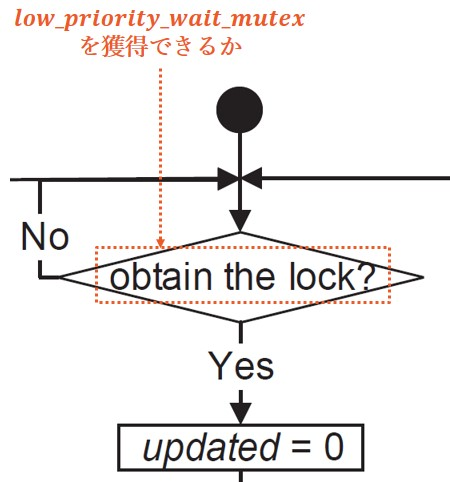
\includegraphics{figure/workflow1.jpg}
            }
        \end{column}
    \end{columns}
\end{frame}

\begin{frame}{reentrantとmutually exclusiveの違い}
    \begin{itemize}
        \item 再入可能なコールバック グループに属すwait\_set内のコールバックはいつでも選択できる
        \item 対照的に, 相互に排他的な各コールバック グループにはフラグ \alert{can\_be\_taken\_from} があり, そのグループに属すコールバックを選択して実行できるかどうかを示す
        \item グループのコールバックが実行のために選択されると, フラグは false に設定され, コールバックの終了後に true に設定される.
        \item 相互に排他的なコールバック グループに属すコールバックは,  can\_be\_taken\_from が true の場合にのみ選択できる.
        \item それ以外の場合, スレッドはこのコールバックをスキップして次のコールバックに進む
    \end{itemize}
\end{frame}

\begin{frame}{can\_be\_taken\_fromによるワークフロー}
    \centering
    \vspace{\headerheight}
    \adjustbox{max width=\textwidth}{
        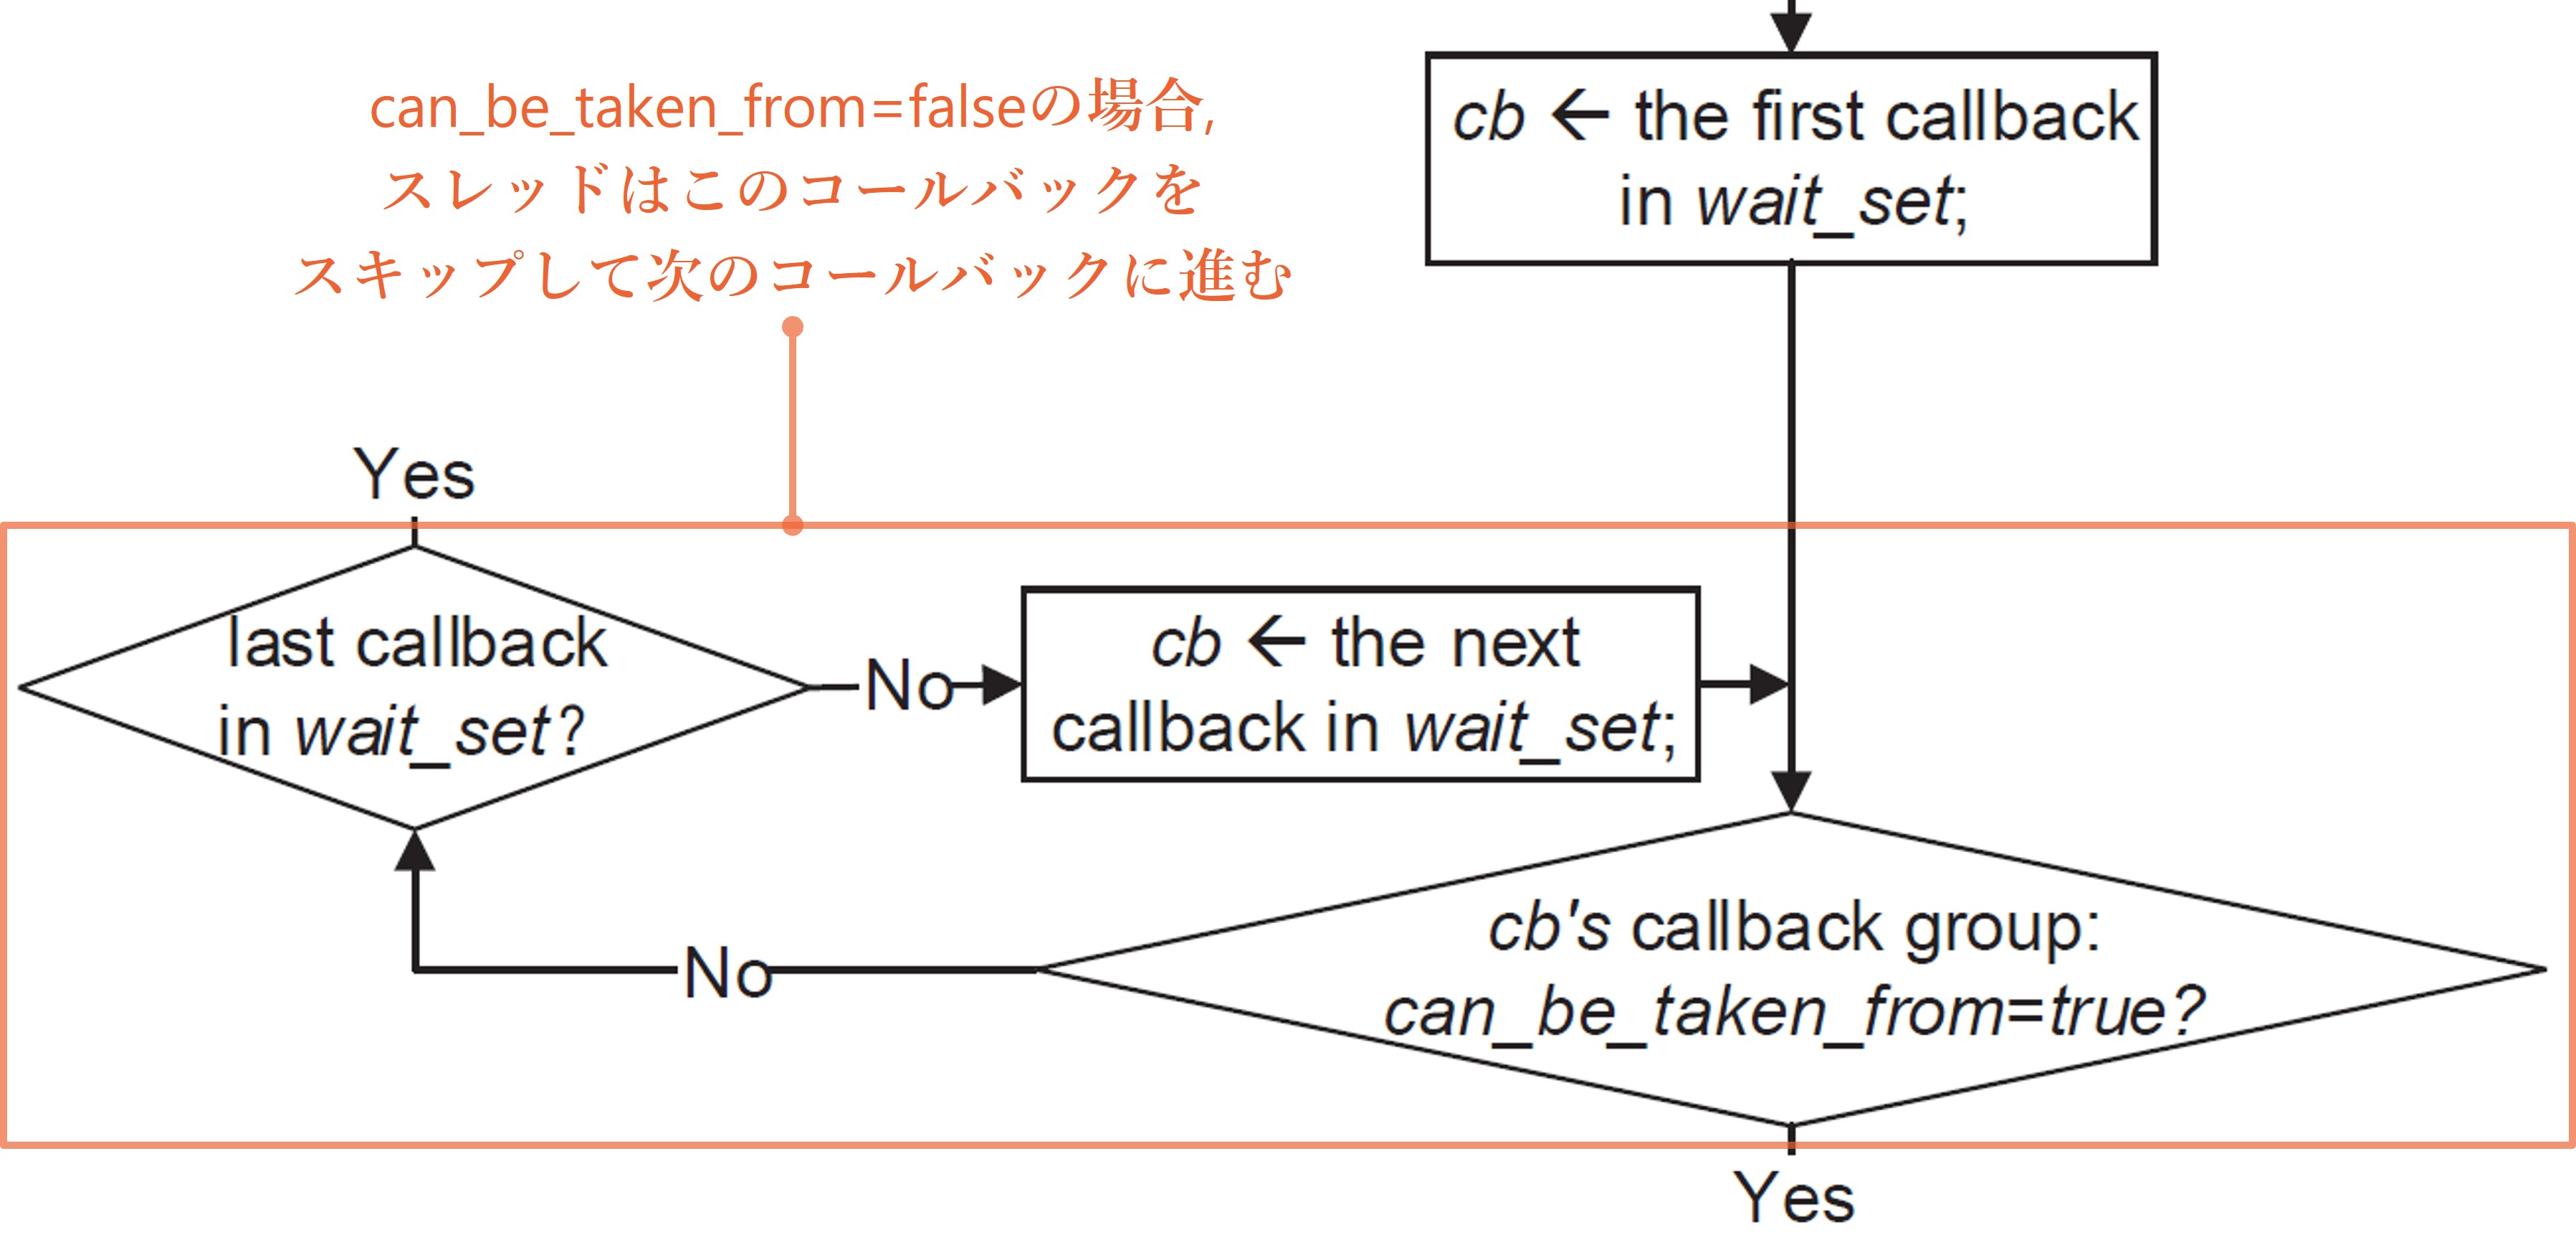
\includegraphics{figure/workflow2.jpg}
    }
\end{frame}

\begin{frame}{コールバック選択後}
    コールバックが正常に選択されると, スレッドは low\_priority\_wait\_mutex をリリースし, wait\_set からコールバックを削除する.

    \centering
    \adjustbox{max width=\textwidth}{
        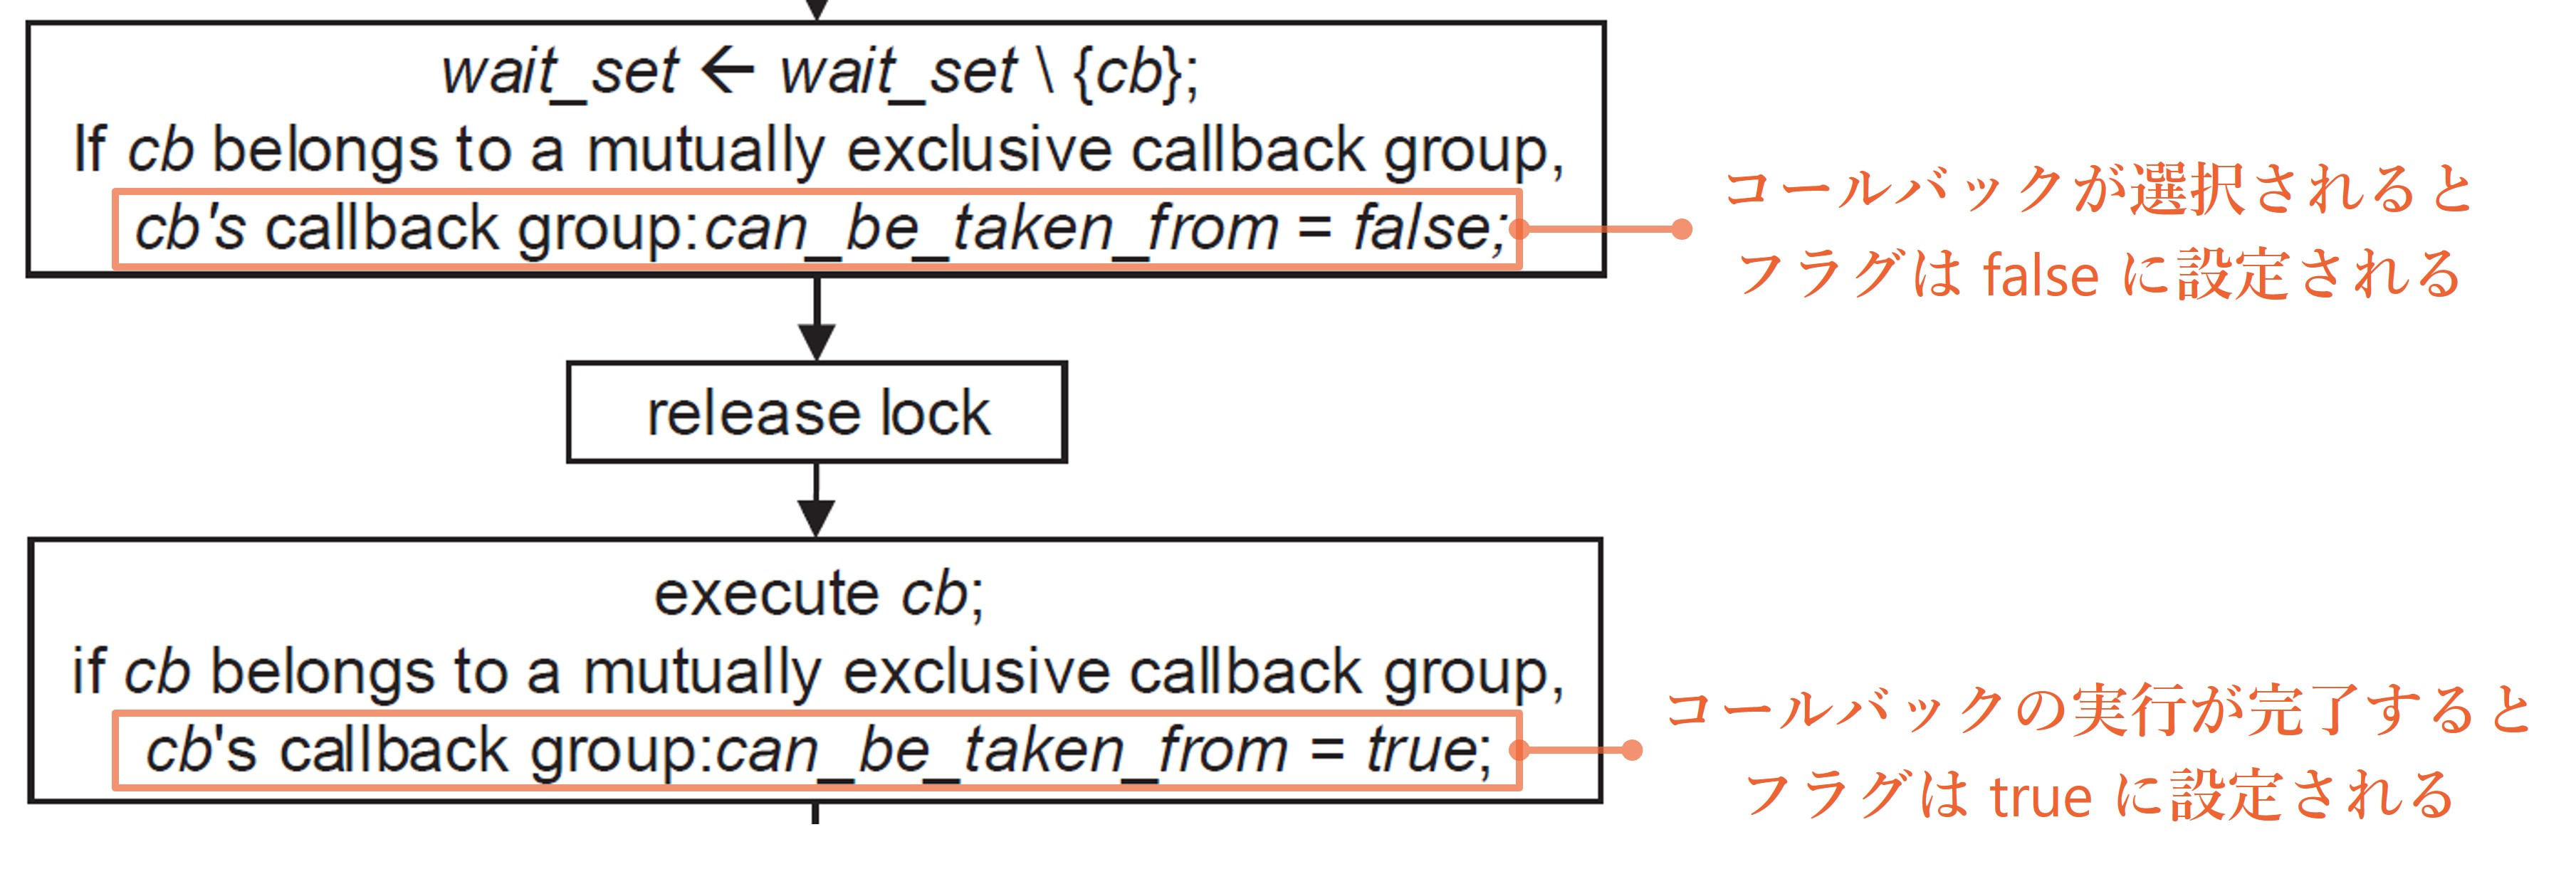
\includegraphics{figure/workflow3.jpg}
    }
\end{frame}

\begin{frame}{yield\_before\_execute}
    \begin{itemize}
        \item yield\_before\_execute の構成が false に設定されている場合, スレッドは選択されたコールバックの実行をすぐに開始する.
        \item それ以外の場合, yield\_before\_execute が true に設定されている場合, スレッドは, 再度スケジュールされるまでプロセッサを OS に譲ります.
        \item この作業では, 既定の構成 yield\_before\_execute $=$ false を考慮する.特に, コールバックは, 最も早く到着したメッセージで非プリエンプティブ\footnote{ROS 2 では, 各コールバックには到着したメッセージをバッファリングするためのキューがあり, その深さはユーザによって指定される [20].簡単にするために, キューが十分に大きく, メッセージが上書きされないと仮定する.}に実行される.
    \end{itemize}
\end{frame}

\begin{frame}{コールバックが選択できない場合}
    \vspace{\headerheight}
    \begin{itemize}
        \item すべてのカテゴリがチェックされ, 実行するコールバックを選択できない場合, スレッドは, wait\_set をリセットし, wait\_set を更新する.
        \item can\_be\_taken\_from が true の場合にのみ, 相互に排他的なコールバック グループからのコールバックを wait\_set に追加できる.
    \end{itemize}

    \centering
    \adjustbox{max width=\textwidth, max height=0.6\textheight}{
        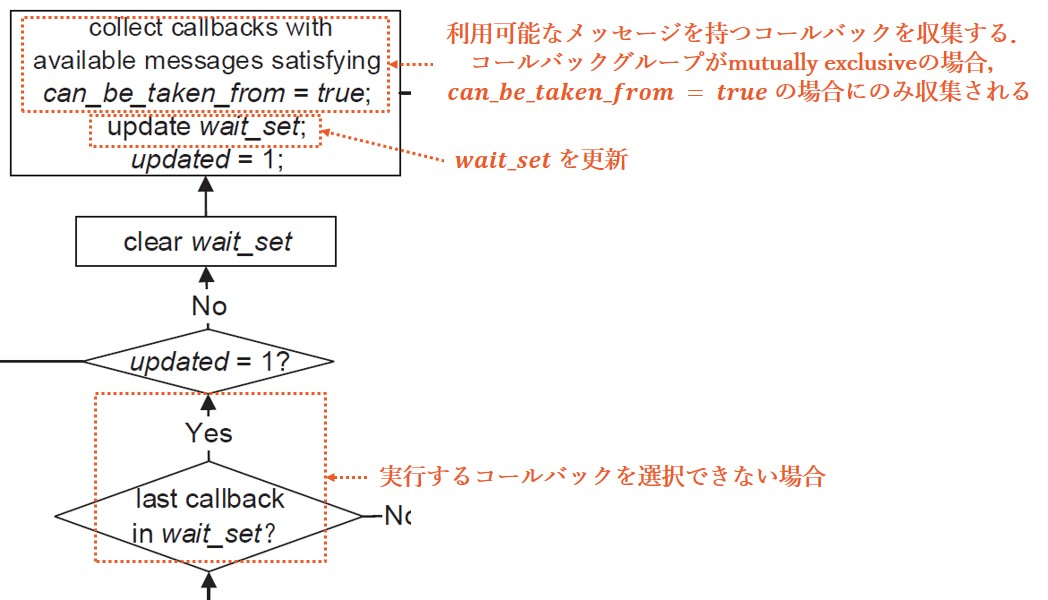
\includegraphics{figure/workflow4.jpg}
    }
\end{frame}

\begin{frame}{コールバックをwait\_setに追加できない場合}
    \begin{itemize}
        \item コールバックを wait\_set に追加できない場合, 頻繁なロックとロック解除によるオーバーヘッドを回避するために, スレッドは, 新しいメッセージの到着によって通知されるか, 定義済みの最大ブロック時間に関してタイムアウトになるまでブロックされる.
        \item それでも実行するコールバックが見つからない場合, スレッドはロックをリリースしてアイドル状態になる.
    \end{itemize}
\end{frame}

\begin{frame}{コールバックをwait\_setに追加できない場合(ワークフロー)}
    \centering
    \vspace{\headerheight}
    \adjustbox{max width=0.9\textwidth}{
        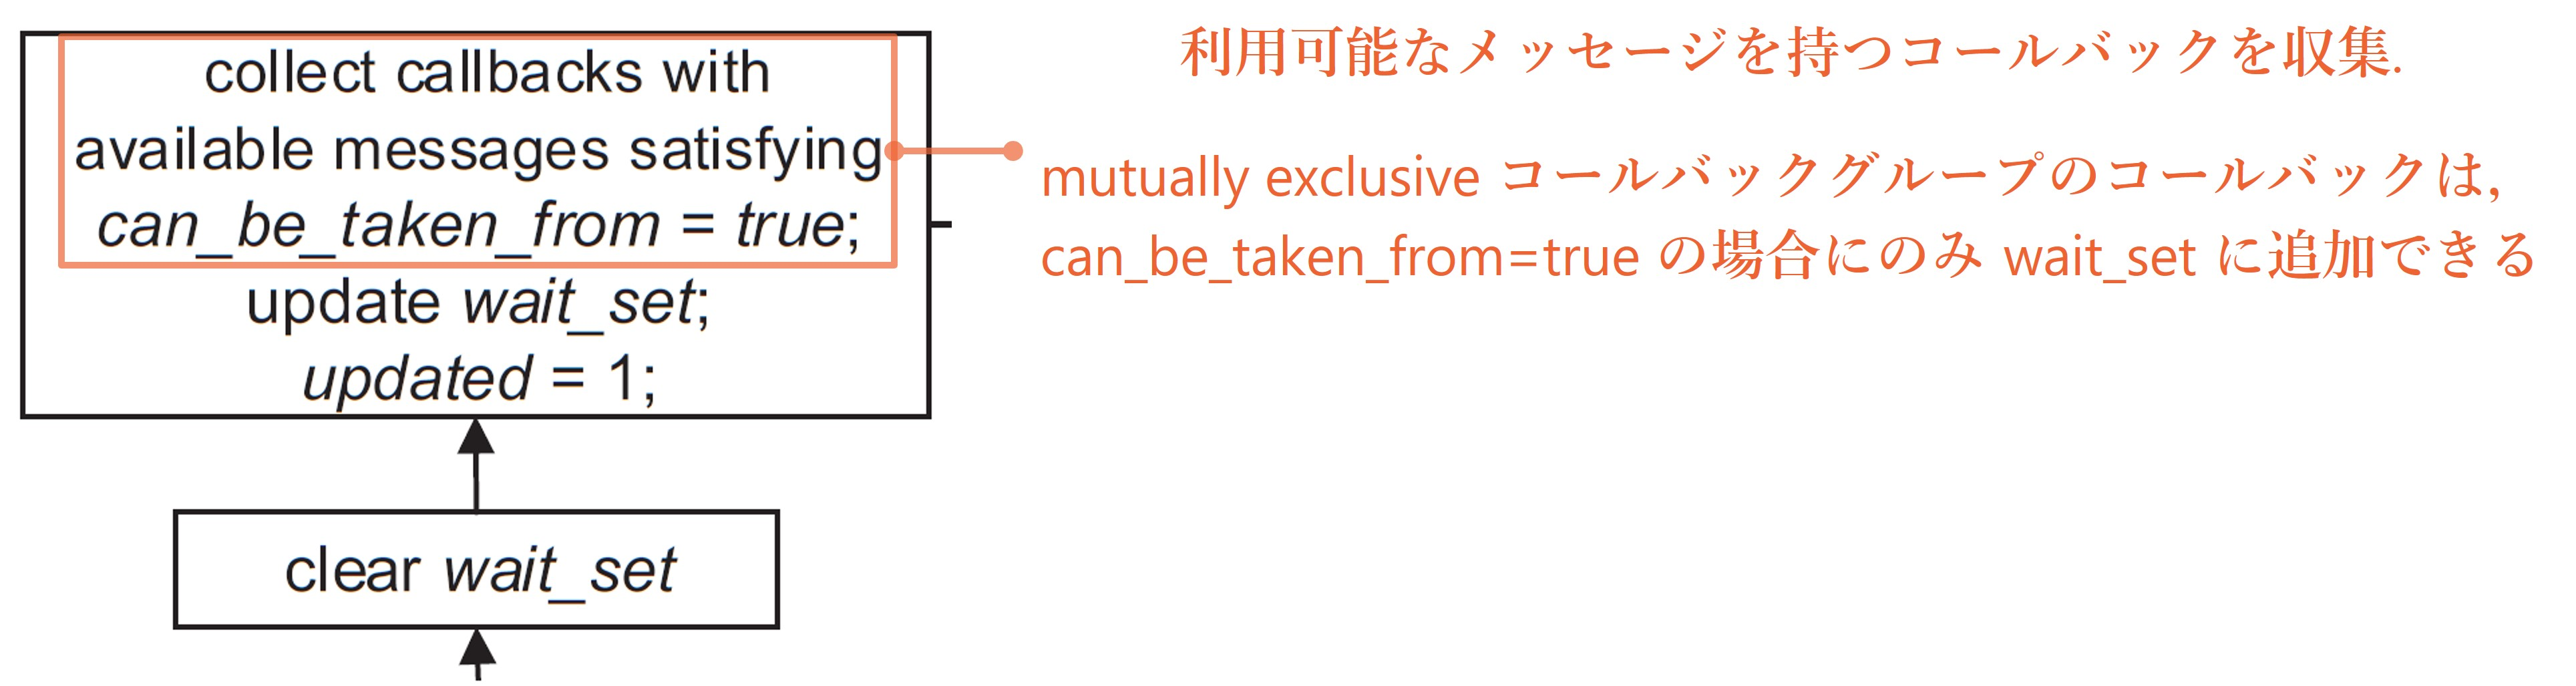
\includegraphics{figure/workflow5.jpg}
    }
\end{frame}
